\question[10] Un carrito de juguete de 1 kg se suelta desde lo alto de una pista sin fricción que se encuentra a la izquierda y rueda fuera de la pista desde una rampa lateral que está a la derecha. El carrito comienza a una altura de 0.80 m, pasa por una vuelta de 0.50 m de diámetro y va por la rampa que tiene una altura de 0.25 m. ¿Cuál es el cambio en la energía potencial gravitacional del carrito de A a B?

\begin{minipage}{0.25\textwidth}
    \begin{figure}[H]
        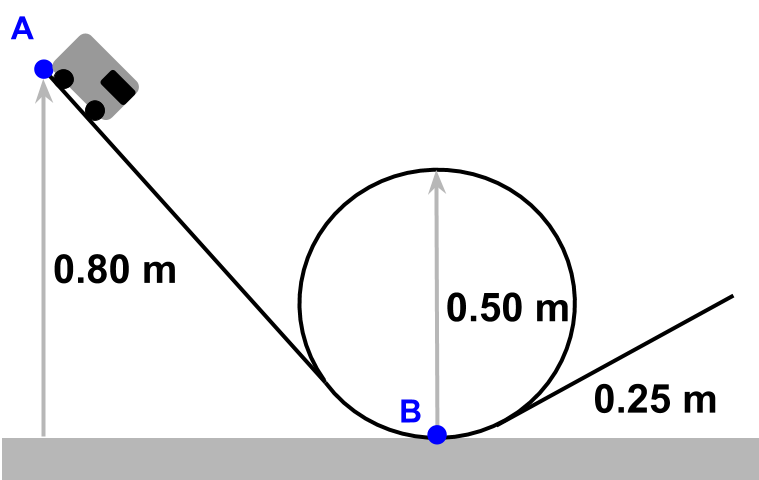
\includegraphics[width=\linewidth]{../images/3bea8730ba0fcd65f1afe168f731639595d83c74.png}
    \end{figure}
\end{minipage}\hfill
\begin{minipage}{0.68\textwidth}
    \begin{solutionbox}{5.2cm}
        \begin{multicols}{2}
            Datos:

            E$_p$ = ?

            h = -0.80 m

            g= 9.8 m/s$^2$

            m = 1 kg

            La energía potencial es:
            \[E_p=mgh\]

            \vspace{1.5cm}

            Sustituyendo nuestros datos en la fórmula:
            \[
                \begin{array}{rl}
                    E_p & = (1 \text{ kg})(9.8 \text{ m/s$^2$})(0.80 \text{ m}) \\[1em]
                        & =-7.84 \text{ J }
                \end{array}
            \]
        \end{multicols}
        \begin{center}El cambio en la energía potencial del carrito del punto A al B es de -7.84 J.\end{center}
    \end{solutionbox}
\end{minipage}